\section{Radiation pressure modeling}

\gls{RP} modeling requires the cooperation of models for the radiation sources and the spacecraft. This section describes a collection of compatible models, starting with a physical description of \gls{RP} and reflectance, then building models of increasing complexity on top of that.

\subsection{Mechanics of radiation pressure}
\label{subsec:general-rp-mechanics}

\gls{RP} results from the momentum transfer between electromagnetic radiation and a surface. A spacecraft may receive such radiation from the Sun but also from other celestial bodies: planets and moons emit albedo radiation through the reflection of sunlight and thermal radiation depending on surface temperature. The \gls{RP} exerts a force on the spacecraft governed by surface properties such as area, reflectivity, and absorptivity. The resulting acceleration is the result of a complex interplay of the bodies emitting radiation (the ``sources'') and the spacecraft receiving the radiation (the ``target'').

Radiation can be characterized by the radiant flux density, which commonly has units of \unit{\irr}. Radiosity is the \emph{emitted and reflected} radiant flux density of an opaque surface. The irradiance $E$ is the \emph{incident} radiant flux density on a surface and provides a convenient way to decouple source and target models: the irradiance and the direction of incidence are sufficient to determine the target acceleration, independent of the actual source. We can combine this information into a vector quantity which we call directional irradiance $\vb E = E \vu r_{t/s}$, where $\vu r_{t/s}$ is the unit vector in the source-to-target direction. One or more directional irradiances, which can be thought of as light rays, are the output of a source model and are used as input to the target model. The \gls{RP} exerted on an irradiated surface is proportional to $1/c$, where $c = \qty{299792458}{m/s}$ is the speed of light. Given the magnitude of $c$, \gls{RP} is usually small (around \qty{4.5e-6}{\N\per\m\squared} for solar radiation at Earth, where $E=\qty{1361}{\irr}$~\cite{Kopp2011}).

Electromagnetic radiation is often composed not just of a single wavelength but rather a range of wavelengths. The distribution can be described by the spectral irradiance in units of \unit{\W\per\square\m\per\Hz}. Since surface properties are often wavelength-dependent, the target model would also have to be aware of the distribution. However, the surface properties as a function of wavelength are often not known, which is also the case for \gls{LRO}. Therefore, we assume the irradiance from source models to be integrated over the whole spectrum and the surface properties of the target model to be valid for all wavelengths.




\subsection{Reflectance distribution}
\label{subsec:general-reflectance-distribution}

Describing the reflectance of a surface is key to \gls{RP} modeling. Both the way a source reflects sunlight and the direction a target is accelerated in depend on the angular distribution of reflectance.

\subsubsection{General reflectance distribution}
In general, reflectance comprises a diffuse (scattered in many directions) and a specular (mirror-like) component. The remaining energy is absorbed by the surface. The reflectance varies with surface normal $\vb N$, incoming radiation direction $\vb L$, and observer direction $\vb V$. This geometry is shown in \cref{fig:reflection-geometry}. A \gls{BRDF} describes the fraction of irradiance reflected toward the observer per steradian, i.e.~\cite{Wetterer2014}
\begin{align}
    f_r (\theta_i, \phi_i, \theta_r, \phi_r)
    = \frac{dL_r(\theta_r, \phi_r)}
    {dE_j(\theta_i, \phi_i)},
\end{align}
where $dL_r$ is the reflected radiance (the directional counterpart to radiosity, typically in \unit{\W\per\square\m\per\steradian}) and $dE_j$ is the received irradiance.

% TODO expand figure with diffuse and specular reflection (e.g. Montenbruck 2000, p. 85)

\begin{figure}[b]
    \centering
    \includegraphics[width=0.8\linewidth]{figures/reflection_geometry.ai}
    \caption{Geometry of a \gls{BRDF} for a surface with normal $\vb N$, incoming direction $\vb L$, and observer direction $\vb V$. The viewing angle $\theta_r$ is between $\vb N$ and $\vb V$. The phase angle (not labeled) is between $\vb L$ and $\vb V$. Adapted from~\cite{Wetterer2014}.}
    \label{fig:reflection-geometry}
\end{figure}

The planetary surface \gls{BRDF} directly leads to the albedo irradiance received by a target if the solar irradiance at the planet's surface and the solid angle subtended by the target are known.

The target surface \gls{BRDF} gives the direction in which the target is accelerated through integration over all directions $\vb V$ in which radiation is reflected. The unitless reaction vector, which includes both the direction and magnitude based on absorbed, specularly reflected, and diffusely reflected fractions, is therefore~\cite{Wetterer2014}
\begin{align}
    \label{eq:brdf-reaction-general}
    \vb R = -\left[ \vb L + \int_{0}^{2\pi} \int_{0}^{\pi/2} f_r \cos\theta_r \vb V d\theta_r d\phi_r \right].
\end{align}
This vector encapsulates the mechanics of momentum transfer. The reaction is minimal for pure absorption ($f_r = 0$) and maximal (double the minimum) for pure specular reflection in the incidence direction.

\subsubsection{Specular--diffuse reflectance distribution}
A simplified \gls{BRDF} is usually more practical for \gls{RP} modeling: the reflectance is assumed to be a mix of an ideal Lambertian diffuse component and a purely mirror-like specular component. Such a \gls{BRDF} is given by~\cite{Wetterer2014}
\begin{align}
    \label{eq:brdf-specular-diffuse}
    f_r = C_d \frac{1}{\pi} + C_s \frac{\delta(\vb V - \vb M)}{\cos \theta_i}
\end{align}
where $C_d$ and $C_s$ are the diffuse and specular reflectivity coefficients. Together with the absorption coefficient $C_a$, energy is conserved when $C_a + C_d + C_s = 1$. The vector $\vb M = 2\cos\theta_i\vb N - \vb L$ is the direction of $\vb L$'s mirror-like reflection, which only contributes if $\vb V = \vb M$.

For this simplified \gls{BRDF}, the integral in \cref{eq:brdf-reaction-general} evaluates analytically to~\cite{Montenbruck2014}
\begin{align}
    \label{eq:brdf-reaction-specular-diffuse}
    \vb R = - \left[ (C_a + C_d) \vb L + \frac{2}{3} C_d \vb N + 2 \cos\theta_i C_s \vb N \right].
\end{align}
If the target is in thermodynamic equilibrium, all absorbed radiation is reradiated instantaneously by Kirchhoff's law. If this reradiation is Lambertian, the reaction vector becomes~\cite{Montenbruck2014}
\begin{align}
    \label{eq:brdf-reaction-specular-diffuse-instrerad}
    \vb R = - \left[ (C_a + C_d) \left(\vb L + \frac{2}{3} \vb N\right) + 2 \cos\theta_i C_s \vb N \right].
\end{align}
The specular contribution is strictly along the surface normal direction since its tangential components cancel. The Lambertian diffuse contribution (both reflected and reradiated) has a component along the incoming direction but also, weighted by a factor $2/3$ (see~\cite{Ziebart2004} for a derivation of this factor), a component along the surface normal. The reaction vector is thus always in the plane spanned by $\vb L$ and $\vb N$.



\subsection{Radiation sources}
\label{subsec:radiation-sources}

Radiation sources emit or reflect radiation, which exerts \gls{RP} onto the target. As explained in \cref{subsec:general-rp-mechanics}, the incident radiation at a target due to a source can be thought of as light rays, which are described by their directional irradiance at the target. How the directional irradiance is calculated depends on the type of source.

\subsubsection{Isotropic point sources}
The simplest source model is a point source that isotropically radiates in all directions. This model is appropriate for far-away sources such as the Sun at \qty{1}{\astronomicalunit} distance. Due to the distance, all rays are effectively parallel and can be merged into a single ray parallel to the source-to-target vector $\vb r_{t/s}$. For an isotropic source, the total luminosity $L$ (units of \unit{\W}) is uniformly distributed over a sphere, leading to an inverse square law. Therefore, the irradiance at the target is
\begin{align}
    \label{eq:irradiance-point-luminosity}
    E = \frac{L}{4\pi\norm{\vb r_{t/s}}^2}.
\end{align}
Alternatively, a reference irradiance $E_\textnormal{ref}$ observed at a distance $\vb r_\textnormal{ref}$ can be scaled:
\begin{align}
    E = E_\textnormal{ref} \frac{r_\textnormal{ref}}{\norm{\vb r_{t/s}}^2}.
\end{align}
The solar luminosity is \qty{3.828e26}{\W}~\cite{Prsa2016}, which corresponds to an irradiance of \qty{1361}{\irr} at \qty{1}{\astronomicalunit}. Note that these values are averages, which vary with the 11-year solar cycle by about \qty{0.1}{\percent} and more on shorter timescales due to sunspot darkening and facular brightening~\cite{Kopp2016}. Observational time series exist to account for these variations~\cite{Dewitte2017}.

\subsubsection{Paneled sources: Discretization}
Radiation due to planets and moons requires more involved source models. Planetary emissions comprise reflected solar radiation and thermal infrared radiation~\cite{Knocke1988}. The fraction of reflected sunlight is called albedo\footnote{Two types of albedo exist: spherical/Bond albedo is the fraction of sunlight reflected in all directions, while geometrical albedo is the fraction of sunlight reflected with respect to an ideal diffuse surface for normal incidence and viewing directions~\cite{Heiken1991}. For our purpose, spherical albedo is appropriate and synonymous with albedo in this paper.} $a$; the corresponding type is therefore also called albedo radiation. Thermal radiation is due to absorbed solar energy that is re-emitted in a delayed fashion. Observation time series of albedo and thermal fluxes exist for Earth~\cite{Dewitte2017}, but physical modeling is required for the Moon.

Since planetary radiation is not isotropic and the spacecraft is typically much closer to the body than to the Sun, the source extent has to be considered. In contrast to the previously described point source, we, therefore, model Earth and Moon as extended sources. These are discretized into sub-sources, from which rays emanate that are, in general, not parallel. The sub-sources can be thought of as panels with an area, orientation, position, and radiosity model. The panel extent is represented by the area but any other panel properties are only evaluated at its center. A panel only radiates from the positive normal side, not from the backside.

Different algorithms exist to divide the planet ellipsoid into panels. Some authors use a longitude--latitude grid (e.g.,~\cite{RodriguezSolano2011a,Woeske2019}, particularly with observed fluxes) or generate static, uniformly spaced panels over the whole sphere (e.g.,~\cite{Wetterer2014}). However, both approaches are inefficient for low-altitude spacecraft, which require a large number of panels, most of which are never visible. Therefore, the de-facto standard is the dynamic\footnote{Dynamic refers to the fact that panels move with the spacecraft, as opposed to static paneling, for which panels are invariant with spacecraft position or time.} paneling method introduced by \citeauthor{Knocke1988}~\cite{Knocke1988}.

% TODO expand: describe Knocke paneling in detail, with figure for zeta, beta...

In Knocke's method, only the visible area of the planet is paneled. This area is a spherical cap, centered at the subsatellite point and divided into concentric rings that are, again, divided into equal-area segments. A central panel is located at the subsatellite point. All panels contribute to the irradiance received by the target. However, the effective area of each panel is projected by its viewing angle $\theta_r$ (see \cref{fig:reflection-geometry}) and the irradiance is attenuated by an inverse square law. In Knocke's method, the rings are spaced such that each panel has the same projected, attenuated area. The projected, attenuated area of a panel is defined as~\cite{Knocke1988}
\begin{align}
    \frac{\dd{A} \cos \theta_r}{\norm{\vb r_{t/s}}^2},
\end{align}
where $\dd{A}$ is the geometric panel area and $r_{t/s}$ is the source-to-target vector (in this case, the panel-to-target vector). More rings and more panels per ring improve the fidelity of the calculated irradiance, barring the resolution limit of the radiosity model (e.g., the albedo distribution). While arbitrary numbers of panels per ring are possible, Knocke suggests multiples of 6 (i.e., six panels in the first ring, twelve panels in the second ring, \dots). The algorithm is elaborated in~\cite{Knocke1989}.

\begin{figure*}[t]
    \centering

    \begin{subfigure}[c]{0.49\textwidth}
        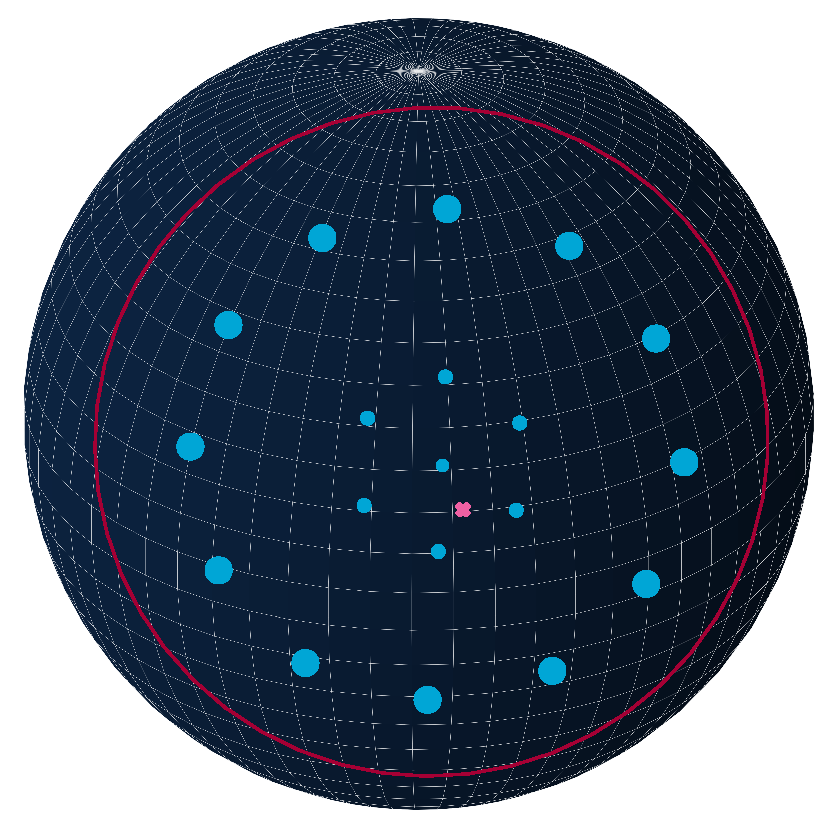
\includegraphics[width=\textwidth]{figures/plots/knocke_paneling_high.pdf}
        \subcaption{High altitude: $h = \qty{1500}{\km}$, 2 rings, angular diameter of cap = \ang{115}.}
    \end{subfigure}
   \hfill
    \begin{subfigure}[c]{0.49\textwidth}
        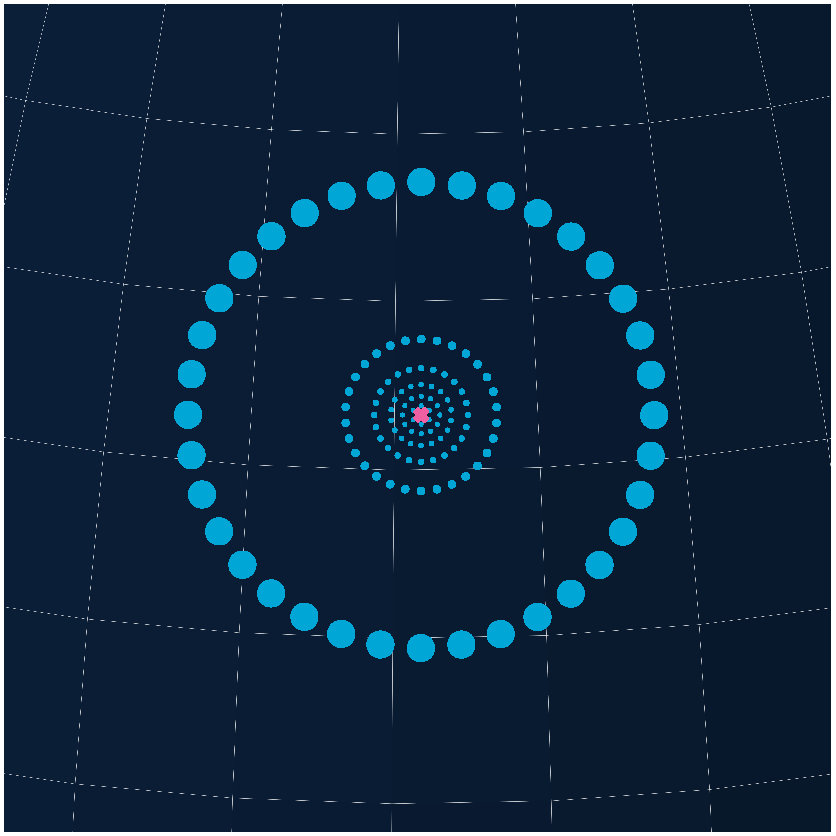
\includegraphics[width=\textwidth]{figures/plots/knocke_paneling_low.pdf}
        \subcaption{Low altitude: $h = \qty{50}{\km}$, 6 rings, angular diameter of cap = \ang{27}.}
        \label{fig:general-knocke-paneling-low}
    \end{subfigure}

   \caption{Panels generated with Knocke's algorithm for the Moon, which has a mean radius of \qty{1737}{\km}. The spacecraft (\textcolor{mpl-pink}{\ding{54}}) sees a spherical cap (\textcolor{mpl-red}{\textbf{---}}), which contains rings of panels and is larger at higher altitudes $h$. Panel centers (\textcolor{mpl-lightblue}{\ding{108}}) are scaled proportional to the panel area. The panels have equal projected, attenuated areas and are therefore concentrated around the subsatellite point. The scenario in \protect\subref{fig:general-knocke-paneling-low} corresponds to LRO's orbit and the paneling used in this paper.}
   \label{fig:general-knocke-paneling}
\end{figure*}

Two examples at different spacecraft altitudes and with different ring numbers are shown in \cref{fig:general-knocke-paneling}. At higher altitudes, a larger area is visible (approaching a hemisphere) and panels are somewhat more uniform in area. At lower altitudes, the panels are more tightly spaced toward the subsatellite point. In both cases, panel areas increase toward the edge of the visible cap. This pattern is a result of the equal projected, attenuated areas.

\subsubsection{Paneled sources: Radiosity models}
The emitted and reflected fluxes of a panel are described by a radiosity model. The irradiance at the target position can then be derived from the panel radiosity. Both radiosity and irradiance commonly have units of \unit{\irr}. Each panel can have one or more radiosity models, usually one for albedo radiation and one for thermal radiation. We present three such models.

The albedo radiosity model accounts for diffuse Lambertian reflection of solar radiation. It implements the specular--diffuse \gls{BRDF} from \cref{eq:brdf-specular-diffuse} with $C_s = 0$ and the albedo value $C_d = a$ at the panel center. The albedo radiosity of a panel is~\cite{Knocke1988}
\begin{align}
    \label{eq:radiosity-albedo}
    J_\textnormal{albedo} = a \left(\cos\theta_i\right)_+ E_s,
\end{align}
where $E_s$ is the incoming solar irradiance at the panel (e.g., as found from \cref{eq:irradiance-point-luminosity}) and the solar incidence angle $\theta_i$ is defined in \cref{fig:reflection-geometry}. The operator $(\cdot)_+$ restricts the input to positive values or zero otherwise. This ensures that no radiation is reflected from the backside.

The delayed thermal radiosity model assumes that absorbed radiation is emitted independently of incident solar radiation and the radiosity is thus not a function of $\theta_i$. The only spatial variations arise from emissivity differences. The emissivity $e$ of a surface is the ratio of the actual radiosity to the ideal black body radiosity. The delay arises from the planet's large thermal inertia. The delayed thermal radiosity of a panel is~\cite{Knocke1988}
\begin{align}
    \label{eq:radiosity-thermal-delayed}
    J_\textnormal{thermal} = e \frac{E_s}{4},
\end{align}
where $e$ is the emissivity of the panel, evaluated at its center. The factor 1/4 is the ratio of the absorbing area (a circle) to emitting area (a sphere). The albedo and delayed thermal model were originally used by \citeauthor{Knocke1988} for Earth emissions~\cite{Knocke1988}.

The angle-based thermal radiosity model is more appropriate than the delayed model if the surface experience significant diurnal cooling and heating. The surface temperature is modeled as a function of the solar incidence angle $\theta_i$ and related to the radiosity through the Stefan--Boltzmann law. The surface temperature is interpolated between the minimum and maximum temperatures, $T_\textnormal{min}$ and $T_\textnormal{max}$ as
\begin{align}
    \label{eq:surface-temperature}
    T = \max\left( T_\textnormal{max} \left(\cos\theta_i\right)_+^{1/4}, T_\textnormal{min} \right).
\end{align}
These temperatures typically correspond to the nighttime temperature and the temperature at the subsolar point. The angle-based thermal radiosity of a panel is then~\cite{Lemoine2013}
\begin{align}
    \label{eq:radiosity-thermal-anglebased}
    J_\textnormal{thermal} = e \sigma T^4,
\end{align}
where $T$ is the surface temperature from \cref{eq:surface-temperature} at the panel center and $\sigma = \qty{5.670e-8}{\W\per\m\squared\per\K\tothe{4}}$ is the Stefan--Boltzmann constant. On the dayside, the radiosity is proportional to $T_\textnormal{max}^4\cos\theta_i$. The maximum radiosity of $e \sigma T_\textnormal{max}^4$ is usually larger than the near-constant $e E_s/4$ from \cref{eq:radiosity-thermal-delayed}, but quickly decreases as the panel moves away from the subsolar point (where $\theta_i = \ang{0}$). On the nightside, the thermal radiosity reduces to $e \sigma T_\textnormal{min}^4$.

The albedo and thermal radiosity models depend on the distribution of $a$ and $e$ over the planetary surface. The values may be assumed constant but generally vary with longitude, latitude, and time. Particularly for Earth, seasons and weather greatly affect reflectivity and emissivity~\cite{Goode2001}. Since the Moon lacks seasons, distributions that only vary spatially are appropriate.

To obtain the irradiance at the target due to the panel radiosity, we account for the projected, attenuated area of the source panel and assume that the emissions follow Lambert's cosine law. The irradiance therefore is
\begin{align}
    \label{eq:irradiance-from-radiosity}
    E = \left(\sum_{J_i \in \mathcal{J}} J_i\right) \frac{\dd{A} \left(\cos\theta_r\right)_+}{\pi\norm{\vb r_{t/s}}^2},
\end{align}
where $\mathcal{J}$ is the set of radiosities from any of the previous radiosity models. Usually, a panel has the albedo model and one thermal model. Here, the source-to-target vector $\vb r_{t/s}$ uses the panel center position, not the source body center. The direction $\vu r_{t/s}$ of the corresponding directional irradiance $\vb E = E \vu r_{t/s}$  is therefore not the same for each panel and thus considers the extent of the source. The radiosities $J_i$ in \cref{eq:irradiance-from-radiosity} can be summed since their radiation emanates from the same point, the panel center. Contrarily, the directional irradiances $\vb E$ can generally not be summed since the their  individual directions need to be retained: the reflectance model of the target may be sensitive to the incoming direction of each ray. Therefore, a set of directional radiances $\mathcal{E}$ is handed to the \gls{RP} target model for acceleration calculations.




\subsection{Radiation pressure targets}
\label{subsec:radiation-pressure-targets}

A \gls{RP} target is a body that is accelerated by \gls{RP}. The target model governs how the incident irradiances from point sources and extended sources accelerate the target body.


\subsubsection{Cannonball target}
In its simplest form, a target can be modeled as an isotropic sphere, also referred to as a cannonball. This sphere is characterized by a cross-sectional area $A_c$ (independent of orientation), radiation pressure coefficient $C_r$ (incorporating reflectivity and absorption coefficients), and mass $m$. Due to its isotropy, any lateral components cancel and the net acceleration is always along the source-to-target vector. The \gls{RP} acceleration of a cannonball target is~\cite{Montenbruck2000}
\begin{align}
    \label{eq:cannonball-target}
    \vb a = C_r \frac{A_c}{m}\sum_{\vb E_j \in \mathcal{E}}\frac{\vb E_j}{c},
\end{align}
where the sum is vectorial and $\sum\vb E_j/c$ is the total \gls{RP} as described in \cref{subsec:general-rp-mechanics}. $\mathcal{E}$ is the set of directional irradiances from any number of sources, both point (\cref{eq:irradiance-point-luminosity}) and paneled (\cref{eq:irradiance-from-radiosity}). The dependence on the area-to-mass ratio $A_c/m$ is similar to drag accelerations. While the cannonball model cannot account for complex geometry, it is often used in orbit determination with $C_r$ as estimated variable. Ray tracing of a detailed model can also be used to establish the evolution of $A_c$ and $C_r$~\cite{Hattori2019}.


\subsubsection{Paneled target}
In reality, the cross-section and optical properties of a spacecraft change with orientation and incident direction. This effect is particularly noticeable for solar panels, which are large and usually track the Sun. To account for the geometry and differences in materials, a spacecraft can be represented as a collection of $n$ panels. Each panel is characterized by its area, surface normal, and reflectance distribution. The position would only be relevant for rotational but not for linear accelerations. In the case of moving parts, the surface normal may change over time. The reflectance distribution can be given as generic \gls{BRDF}, but is often a specular--diffuse \gls{BRDF}. The \gls{RP} acceleration of a paneled target is~\cite{Marshall1992}
\begin{align}
    \label{eq:paneled-target}
    \vb a = \frac{1}{m} \sum_{\vb E_j \in \mathcal{E}} \left( \frac{\norm{\vb E_j}}{c} \sum_{k=1}^n A_k \left(\cos\theta_{i,k}\right)_+ \vb R_k\right),
\end{align}
where the indices $j$ and $k$ denote the (sub-)source and target panel, respectively. $A_k$ is the area of the $k$-th panel. $\theta_{i,k}$ is the incidence angle of $\vb E_i$ onto the $k$-th panel. $\vb R_k$ is the reaction vector as defined by {\renewcommand\creflastconjunction{ or }\cref{eq:brdf-reaction-general,eq:brdf-reaction-specular-diffuse,eq:brdf-reaction-specular-diffuse-instrerad}}, depending on the \gls{BRDF}. The reaction vector is a function of the panel surface normal $\vb N$ and the source-to-target direction $\vb L = \vu E_j$. Therefore, the inner sum has to be evaluated for each directional irradiance $\vb E_j$ of the outer sum. However, $\vb E_j$ itself is only calculated once for all panels at the target center to avoid quadratic computational complexity. In general, the resulting acceleration is not along the source-to-target direction as for the cannonball.

Extensions for the paneled target model exist. The model described above does not account for self-shadowing, which occurs when one ray would intersect two panels. This effectively reduces the area of the shadowed panel, an effect that can be significant for complex spacecraft geometries~\cite{Mazarico2009}. Polygon intersections enable simple calculation of the effective area~\cite{Mazarico2009}. Ray tracing is more involved but can also account for multiple reflections between target panels~\cite{Kenneally2020}.

Another extension is the radiation pressure due to the thermal radiation of the spacecraft itself. Instantaneous reradiation as modeled by \cref{eq:brdf-reaction-specular-diffuse-instrerad} for the case of thermodynamic equilibrium is a simple version of this. In reality, panels heat up and cool down (particularly during eclipses) through radiation, conduction, and internal heat production. Advanced models, therefore, calculate the temperature of each panel. Such models range from a simple heat balance~\cite{Wetterer2014} to finite element models~\cite{Woeske2019}. However, a lack of knowledge of the thermal properties may restrict the applicability. For the sake of simplicity, neither self-shadowing nor thermal radiation pressure of the spacecraft are considered in this paper.

% TODO expand add figure how symbols fit together


\subsection{Occultation}
All previous models assume that the line of sight between the the source and the target is unobstructed. However, occultation is a common astronomical phenomenon: a low-altitude spacecraft may be in the planet's shadow for more than a third of its orbit, and partial or full lunar eclipses can occur multiple times per year. We present two occultation models.


\begin{figure}[t]
    \centering
    \includegraphics[width=\linewidth]{figures/eclipse_geometry.ai}
    \caption{Conical occultation model for spherical sources and occulting bodies. The observer is partially illuminated in the penumbra but fully shadowed in the umbra. Adapted from~\cite{Vallado2013}.}
    \label{fig:eclipse-geometry}
\end{figure}

\subsubsection{Shadow function}
The shadow function $\nu$ describes the fraction of light received from a spherical source in the presence of an occulting spherical body. The geometry of the conical occultation model is shown in \cref{fig:eclipse-geometry}. In the umbra, the source is fully occulted and the observer does not receive any radiation ($\nu = 0$), a state referred to as total eclipse. In the penumbra, the observer can see part of the source ($0 < \nu < 1$). Only outside the shadow region does the observer receive the full radiation ($\nu = 1$). In the case of a lunar eclipse, Earth occults the Sun and casts a shadow onto the Moon such that there is no lunar albedo radiation. On the nightside of a planet, the planet itself occults the Sun.

With the models described in \cref{subsec:radiation-sources,subsec:radiation-pressure-targets}, the shadow function needs to be considered for radiation from a point source, both when directly incident on the target and when used as solar radiation for albedo radiosity. The extent of the source and occulting bodies needs to be known for shadow function calculations, even in the case of point sources. A derivation of the conical model for $\nu$ is presented by \citeauthor{Montenbruck2000}~\cite{Montenbruck2000}.

The conical model can only account for one occulting body. In the case of multiple occulting bodies, shadows might overlap and the product of their shadow functions would underestimate the actual received fraction. Knowledge of the shadow intersection would be required to avoid this. \citeauthor{Zhang2019} derived a model for two occulting bodies~\cite{Zhang2019}. However, only single occultations are considered in this paper.

More involved shadow models exist that improve the prediction of the penumbra passage. These models can consider planetary oblateness and atmospheric effects like absorption, scattering, and refraction~\cite{Li2019}. Other models can account for topography by combining a paneled Sun model with a topography map~\cite{Mazarico2018}. These modifications usually prolong the penumbra duration.


\subsubsection{Point-to-point visibility}
For source panels represented by their center point, the shadow function becomes binary: either there is a line of sight between the panel center and the target or there is not. Such point-to-point visibility with a spherical occulting body is easily modeled geometrically. A derivation is given by \citeauthor{Vallado2013}~\cite{Vallado2013}. Multiple occultations are supported in this occultation model by the logical conjunction of the individual visibilities.
